\section{Time evolution}
Thanks to the data collected, we have the state of the system for each instant of time, and we are able to analyze the temporal evolution of the system. In this graph we have considered radius 75 and probabity 0,3 inside the 200 nodes case.
\begin{figure}[H]
\centering
    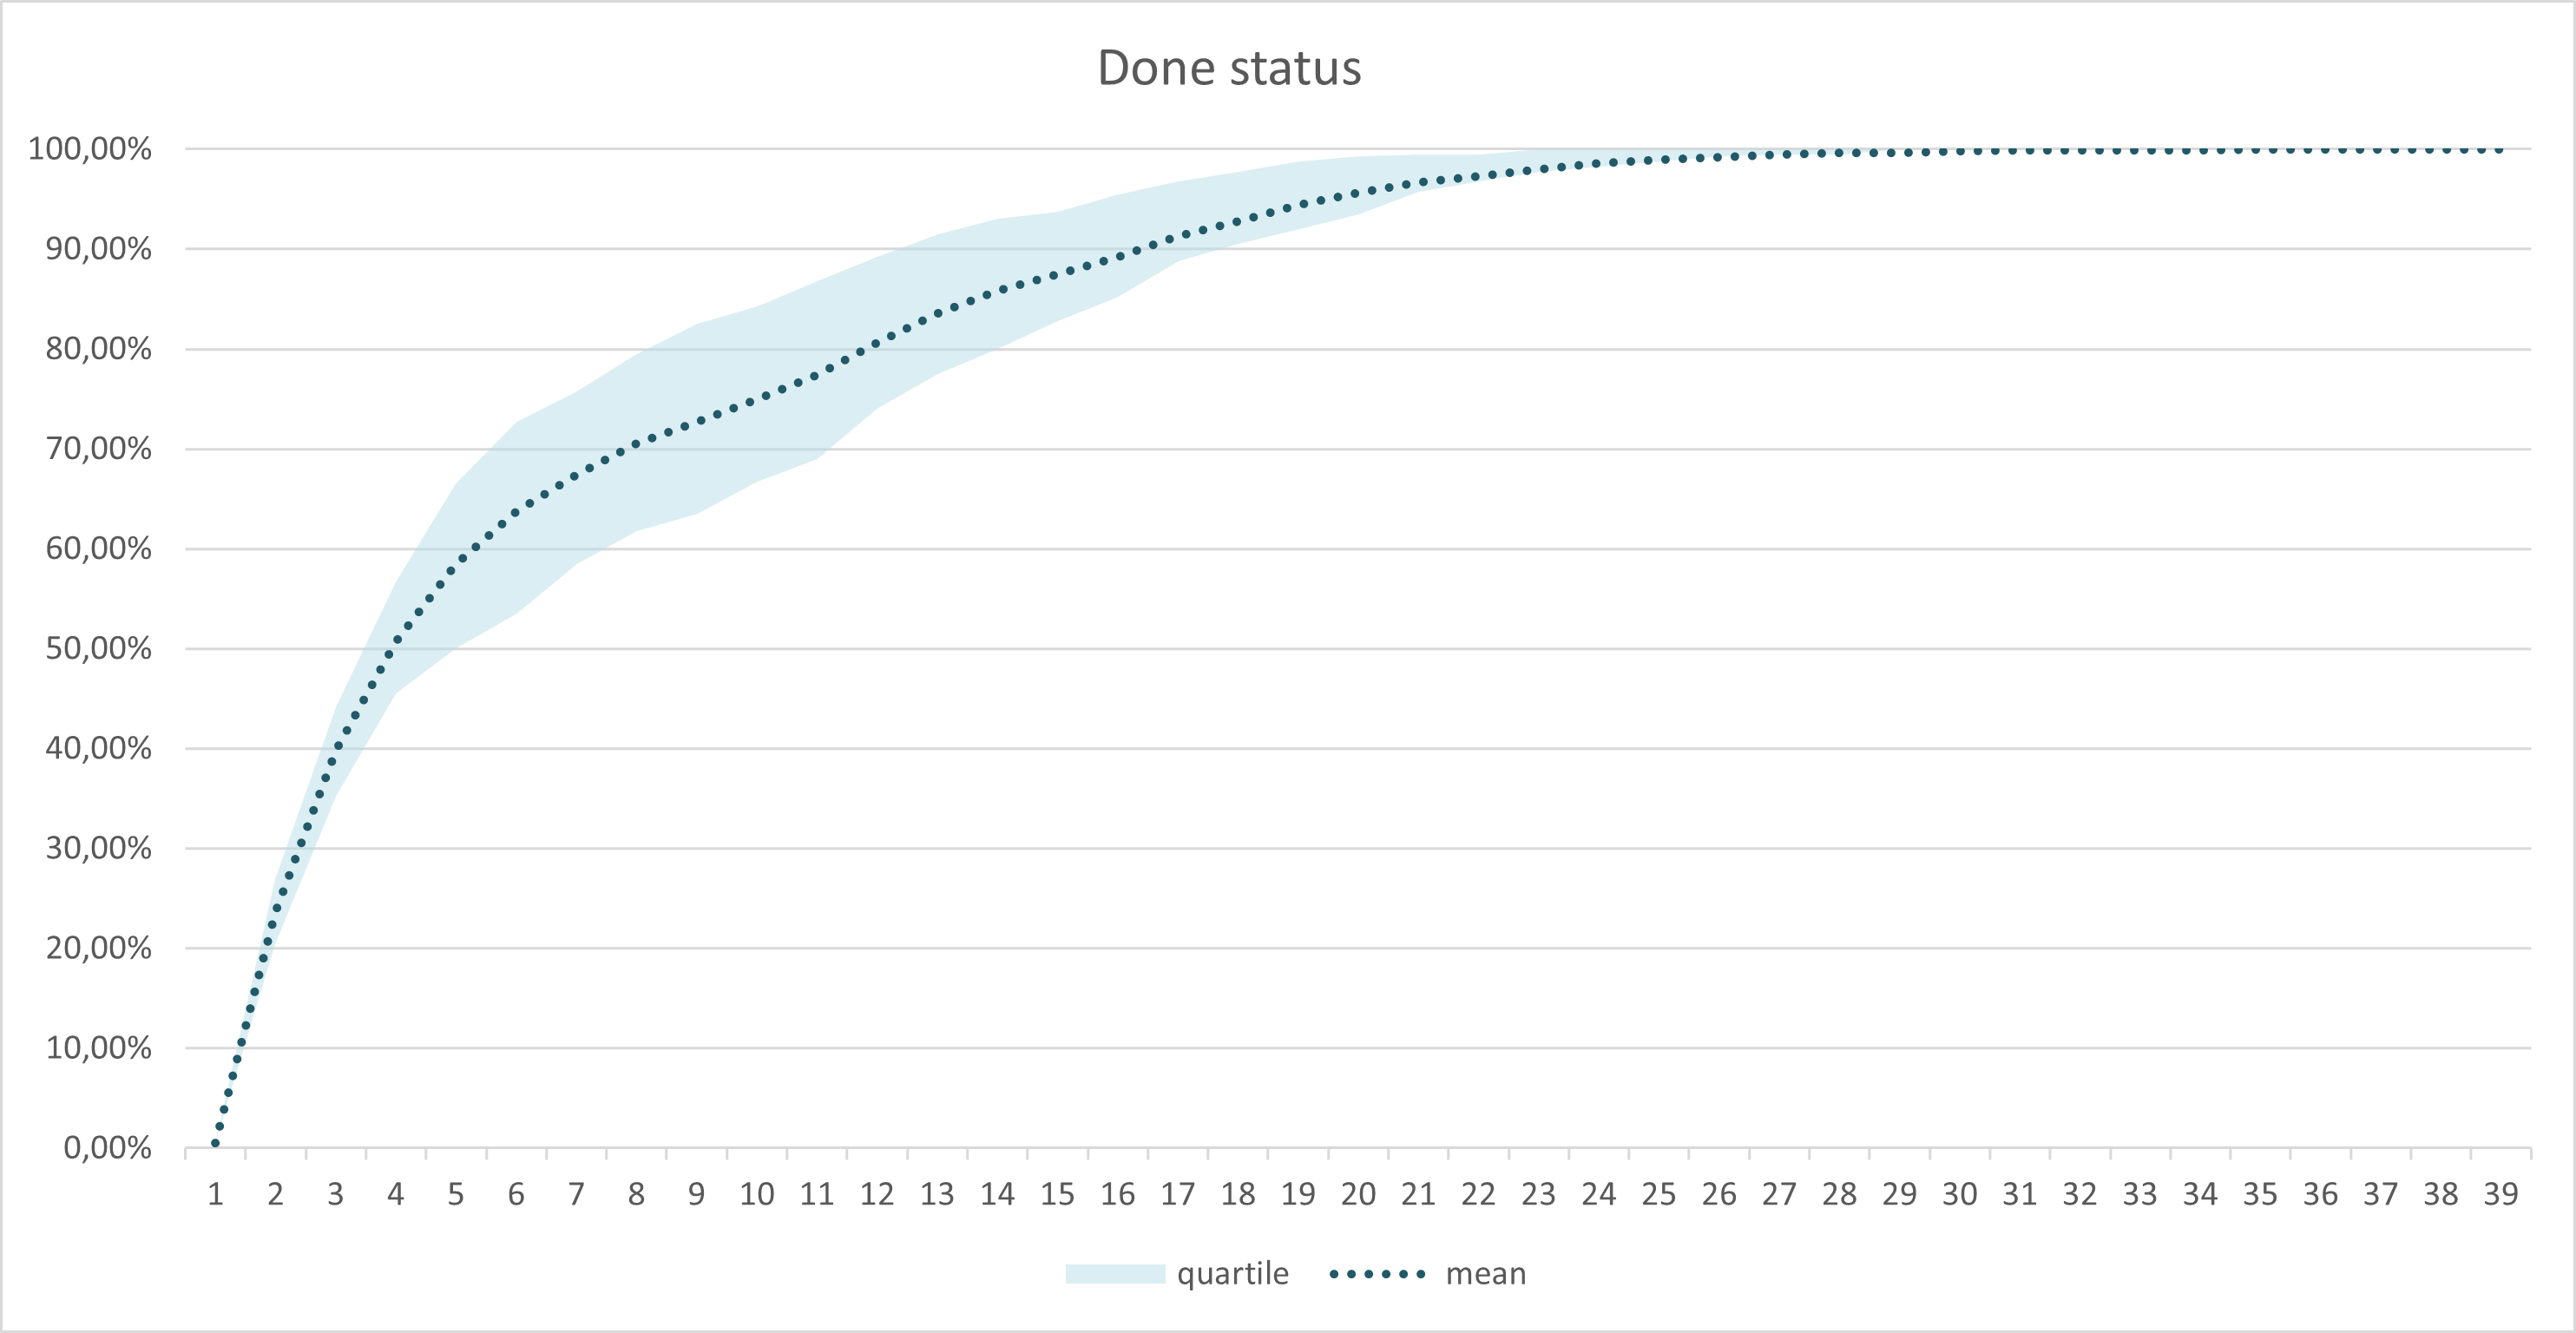
\includegraphics[width= 1\textwidth]{./images/DoneStatus_200N-30p75r.png}
    \caption{Done status}
    \label{fig:immagine}
\end{figure}